%%%%%%%%%%%%%%%%%%%%%%%%%%%%%%%%%%%%%%%%%%%%%%%%%%%%%%%%%%%%%%%%%%%%%%
%%  Copyright by Wenliang Du.                                       %%
%%  This work is licensed under the Creative Commons                %%
%%  Attribution-NonCommercial-ShareAlike 4.0 International License. %%
%%  To view a copy of this license, visit                           %%
%%  http://creativecommons.org/licenses/by-nc-sa/4.0/.              %%
%%%%%%%%%%%%%%%%%%%%%%%%%%%%%%%%%%%%%%%%%%%%%%%%%%%%%%%%%%%%%%%%%%%%%%

\newcommand{\commonfolder}{../../common-files}
\newcommand{\webcommon}{../Web_Common}

\documentclass[11pt]{article}

\usepackage[most]{tcolorbox}
\usepackage{times}
\usepackage{epsf}
\usepackage{epsfig}
\usepackage{amsmath, alltt, amssymb, xspace}
\usepackage{wrapfig}
\usepackage{fancyhdr}
\usepackage{url}
\usepackage{verbatim}
\usepackage{fancyvrb}
\usepackage{adjustbox}
\usepackage{listings}
\usepackage{color}
\usepackage{subfigure}
\usepackage{cite}
\usepackage{sidecap}
\usepackage{pifont}
\usepackage{mdframed}
\usepackage{textcomp}
\usepackage{enumitem}


% Horizontal alignment
\topmargin      -0.50in  % distance to headers
\oddsidemargin  0.0in
\evensidemargin 0.0in
\textwidth      6.5in
\textheight     8.9in 

\newcommand{\todo}[1]{
\vspace{0.1in}
\fbox{\parbox{6in}{TODO: #1}}
\vspace{0.1in}
}


\newcommand{\unix}{{\tt Unix}\xspace}
\newcommand{\linux}{{\tt Linux}\xspace}
\newcommand{\minix}{{\tt Minix}\xspace}
\newcommand{\ubuntu}{{\tt Ubuntu}\xspace}
\newcommand{\setuid}{{\tt Set-UID}\xspace}
\newcommand{\openssl} {\texttt{openssl}}


\pagestyle{fancy}
\lhead{\bfseries SEED Labs}
\chead{}
\rhead{\small \thepage}
\lfoot{}
\cfoot{}
\rfoot{}


\definecolor{dkgreen}{rgb}{0,0.6,0}
\definecolor{gray}{rgb}{0.5,0.5,0.5}
\definecolor{mauve}{rgb}{0.58,0,0.82}
\definecolor{lightgray}{gray}{0.90}


\lstset{%
  frame=none,
  language=,
  backgroundcolor=\color{lightgray},
  aboveskip=3mm,
  belowskip=3mm,
  showstringspaces=false,
%  columns=flexible,
  basicstyle={\small\ttfamily},
  numbers=none,
  numberstyle=\tiny\color{gray},
  keywordstyle=\color{blue},
  commentstyle=\color{dkgreen},
  stringstyle=\color{mauve},
  breaklines=true,
  breakatwhitespace=true,
  tabsize=3,
  columns=fullflexible,
  keepspaces=true,
  escapeinside={(*@}{@*)}
}

\newcommand{\newnote}[1]{
\vspace{0.1in}
\noindent
\fbox{\parbox{1.0\textwidth}{\textbf{Note:} #1}}
%\vspace{0.1in}
}


%% Submission
\newcommand{\seedsubmission}{You need to submit a detailed lab report, with screenshots,
to describe what you have done and what you have observed.
You also need to provide explanation
to the observations that are interesting or surprising.
Please also list the important code snippets followed by
explanation. Simply attaching code without any explanation will not
receive credits.}

%% Book
\newcommand{\seedbook}{\textit{Computer \& Internet Security: A Hands-on Approach}, 2nd
Edition, by Wenliang Du. See details at \url{https://www.handsonsecurity.net}.}

%% Videos
\newcommand{\seedisvideo}{\textit{Internet Security: A Hands-on Approach},
by Wenliang Du. See details at \url{https://www.handsonsecurity.net/video.html}.}

\newcommand{\seedcsvideo}{\textit{Computer Security: A Hands-on Approach},
by Wenliang Du. See details at \url{https://www.handsonsecurity.net/video.html}.}

%% Lab Environment
\newcommand{\seedenvironment}{This lab has been tested on our pre-built
Ubuntu 16.04 VM, which can be downloaded from the SEED website. }

\newcommand{\seedenvironmentA}{This lab has been tested on our pre-built
Ubuntu 16.04 VM, which can be downloaded from the SEED website. }

\newcommand{\seedenvironmentB}{This lab has been tested on our pre-built
Ubuntu 20.04 VM, which can be downloaded from the SEED website. }

\newcommand{\seedenvironmentAB}{This lab has been tested on our pre-built
Ubuntu 16.04 and 20.04 VMs, which can be downloaded from the SEED website. }

\newcommand{\nodependency}{Since we use containers to set up the lab environment, 
this lab does not depend too much on our SEED VM. You can do this lab
using other VMs or physical machines. }







\newcommand{\seedlabcopyright}[1]{
\vspace{0.1in}
\fbox{\parbox{6in}{\small Copyright \copyright\ {#1}\ \ by Wenliang Du.\\
      This work is licensed under a Creative Commons
      Attribution-NonCommercial-ShareAlike 4.0 International License.
      If you remix, transform, or build upon the material, 
      this copyright notice must be left intact, or reproduced in a way that is reasonable to
      the medium in which the work is being re-published.}}
\vspace{0.1in}
}






\newcommand{\ubuntutwo}{{\tt Ubuntu12.04}\xspace}
\newcommand{\ubuntusix}{{\tt Ubuntu16.04}\xspace}


\lhead{\bfseries SEED Labs -- MD5 Collision Attack Lab}

\def \code#1 {\fbox{\scriptsize{\texttt{#1}}}}

\begin{document}


\newcommand{\mdFigs}{./Figs}

\begin{center}
{\LARGE MD5 Collision Attack Lab}
\end{center}

\seedlabcopyright{2018}




% *******************************************
% SECTION
% ******************************************* 
\section{Introduction}


A secure one-way hash function needs to satisfy two properties: the one-way property and 
the collision-resistance property. The one-way property ensures that given a hash value
\texttt{h}, it is computationally infeasible to find an input $M$, such 
that \texttt{hash($M$) = h}. 
The collision-resistance property ensures that it is computationally 
infeasible to find two
different inputs \texttt{$M_1$} and \texttt{$M_2$}, such that
\texttt{hash($M_1$) = hash($M_2$)}. 


Several widely-used one-way hash functions have trouble maintaining the collision-resistance
property. At the rump session of CRYPTO 2004, Xiaoyun Wang and co-authors demonstrated
a collision attack against MD5~\cite{Black:2006:MD5}.
In February 2017, CWI Amsterdam and Google Research announced
the \textit{SHAttered}\index{SHAttered} attack, which breaks the collision-resistance property
of SHA-1~\cite{shattered}. While many students do not have trouble understanding the importance of
the one-way property, they cannot easily grasp why the collision-resistance property is 
necessary, and what impact these attacks can cause.   


The learning objective of this lab is for students to really
understand the impact of collision attacks, and see in first hand what
damages can be caused if a widely-used one-way hash function's
collision-resistance property is broken. To achieve this goal, students
need to launch actual collision attacks against the MD5 hash function.
Using the attacks, students should be able to create two different programs
that share the same MD5 hash but have completely different behaviors.
This lab covers a number of topics described in the following:

\begin{itemize}[noitemsep]
\item One-way hash function, MD5
\item The collision-resistance property
\item Collision attacks
\end{itemize}


\paragraph{Readings.}
Detailed coverage of the one-way hash function can be found in the following:

\begin{itemize}
\item Chapter 22 of the SEED Book, \seedbook
\end{itemize}



\paragraph{Lab Environment.} \seedenvironmentB \ \ 
The lab uses a tool 
called ``Fast MD5 Collision Generation'', which was written by Marc Stevens. 
The name of the binary is called \texttt{md5collgen} in our VM, and it is 
installed inside the \texttt{/usr/bin} folder. If it is not there, you
can download it from the lab's website (inside \texttt{Labsetup.zip}). 
If you are interested in installing the tool to your own machine, you
can download the source code directly from
\url{https://www.win.tue.nl/hashclash/}.


%\paragraph{Reading Materials.} One-way hash function, its properties,
%applications, and attacks (including the one covered in this lab)
%are explained in great details in Chapter 18 of the
%book \textit{Computer Security: A Hands-on Approach}, written by Wenliang
%Du. 

\paragraph{Acknowledgment} This lab was developed with the help of Vishtasp
Jokhi, a graduate student in the Department of Electrical Engineering and
Computer Science at Syracuse University.

%\newpage


% *******************************************
% SECTION
% ******************************************* 
\section{Lab Tasks}


% -------------------------------------------
% SUBSECTION
% ------------------------------------------- 
\subsection{Task 1: Generating Two Different Files with the Same MD5 Hash}


In this task, we will generate two different files with the same MD5 hash values. 
The beginning parts of these two files need to be the same, i.e., they share the same prefix.
We can achieve this using the \texttt{md5collgen} program, which allows us 
to provide a prefix file with any arbitrary content. 
The way how the program works is illustrated in Figure~\ref{md5:fig:md5collgen}.
The following command generates two output files,
\texttt{out1.bin}  and \texttt{out2.bin}, for a given a prefix file \texttt{prefix.txt}: 

\begin{lstlisting}
$ md5collgen -p prefix.txt -o out1.bin out2.bin
\end{lstlisting}


\begin{figure}[htb]
	\centering
	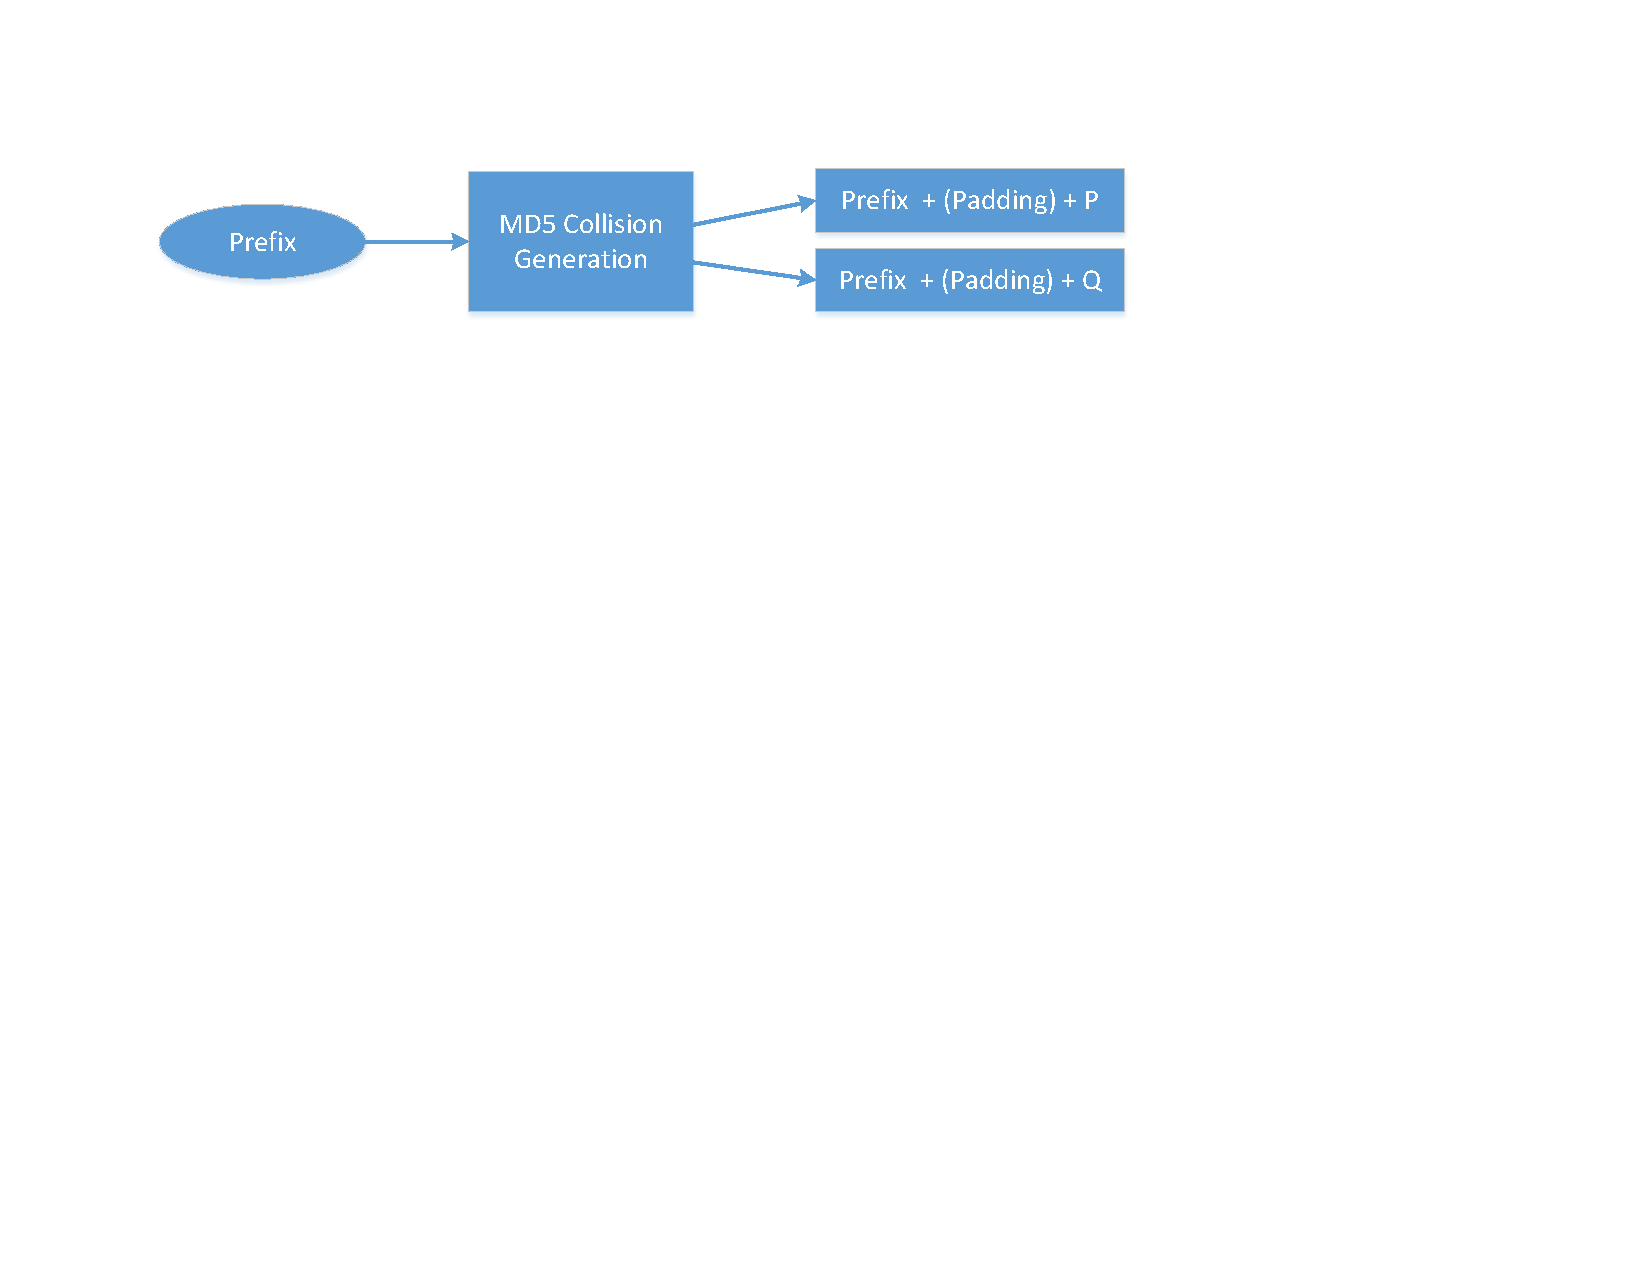
\includegraphics[width=0.8\textwidth]{\mdFigs/generate_collision.pdf}
	\caption{MD5 collision generation from a prefix}
	\label{md5:fig:md5collgen}
\end{figure}
 

We can check whether the output files are distinct or not using the \texttt{diff} command.
We can also use the \texttt{md5sum} command to check the MD5 hash 
of each output file. See the following commands.

\begin{lstlisting}
$ diff out1.bin out2.bin
$ md5sum out1.bin
$ md5sum out2.bin
\end{lstlisting}
 
Since \texttt{out1.bin} and \texttt{out2.bin} are binary, we cannot view them using a text-viewer
program, such as \texttt{cat} or \texttt{more}; 
we need to use a binary editor to view (and edit) them. We have already installed a hex editor software
called \texttt{bless} in our VM. Please use such an editor to view these two output files, and
describe your observations. In addition, you should answer the following questions:


\begin{itemize}[label={--}]
\item \textbf{Question 1.} If the length of your prefix file is not multiple of 64, what is going to
happen?  

\item \textbf{Question 2.} Create a prefix file with exactly 64 bytes, and run the collision tool
again, and see what happens. 

\item \textbf{Question 3.} Are the data (128 bytes) generated by \texttt{md5collgen} completely 
different for the two output files? Please identify all the bytes that are different. 
\end{itemize}
 

%If the same hash is generated by the above two commands, the program was successful and an MD5
%collision was generated.  If we use a hex editor to view the two output files generated
%previously, we can see that the beginning of both the files have the same prefix as specified
%in the prefix file. They also have 128 bytes of data which is appended to the prefix. The 128
%bytes of binary data added to each file is different for both files, and this is the part
%generated by the program which produces the MD5 collision.




% -------------------------------------------
% SUBSECTION
% ------------------------------------------- 
\subsection{Task 2: Understanding MD5's Property}


In this task, we will try to understand some of the properties of the
MD5 algorithm. These properties are important for us to conduct further tasks in this lab. 
MD5 is a quite complicated algorithm, but from very high level, it 
is not so complicated. 
As Figure~\ref{md5:fig:how_md5_works} shows, 
MD5 divides the input data into blocks of 64 bytes, and then computes the hash 
iteratively on these blocks. The core of the MD5 algorithm is a compression function, 
which takes two inputs, a 64-byte data block and the
outcome of the previous iteration. The compression function
produces a 128-bit IHV, which stands for ``Intermediate Hash Value'';
this output is then fed into the next iteration. If the current
iteration is the last one, the IHV will be the final hash value. 
The IHV input for the first iteration (IHV$_0$) is a fixed value. 


\begin{figure}[htb]
	\centering
	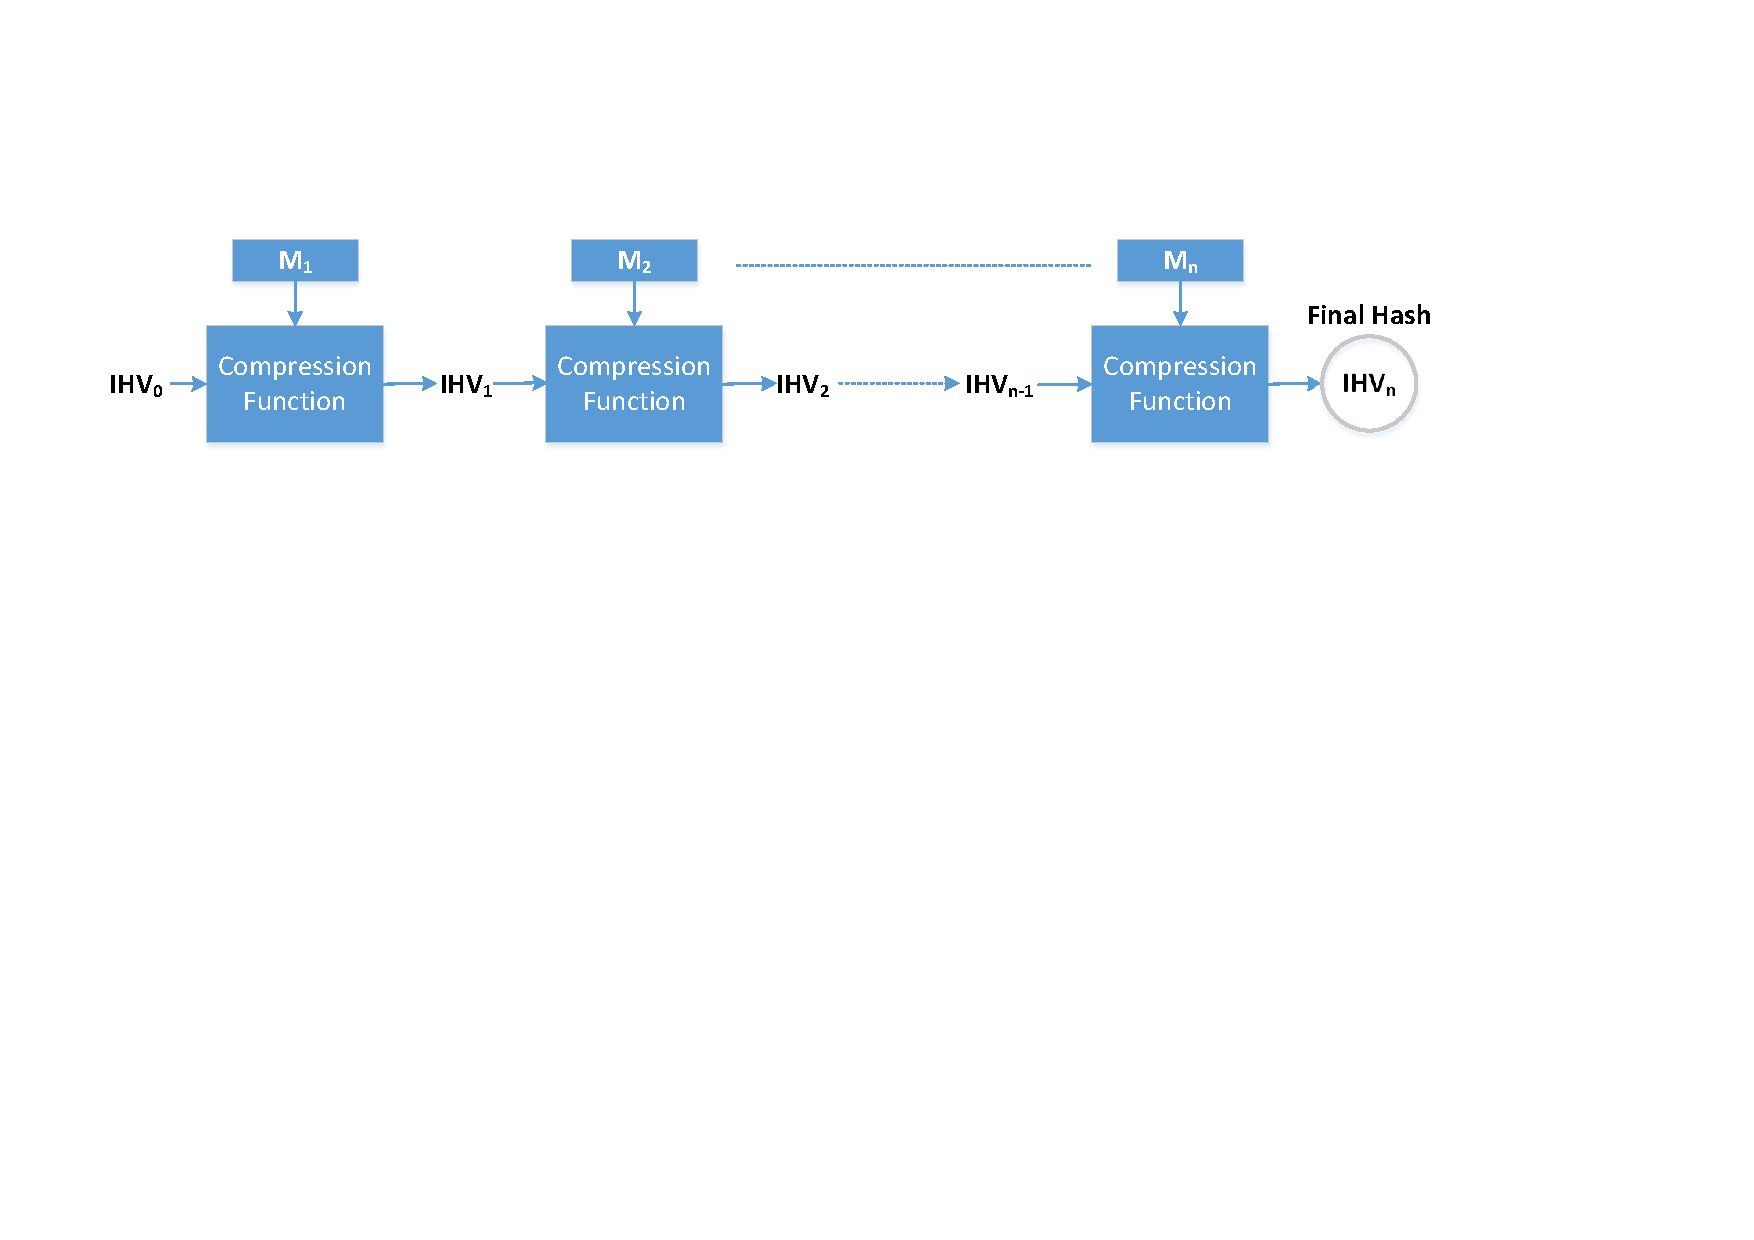
\includegraphics[width=0.90\textwidth]{\mdFigs/How_MD5_works.pdf}
	\caption{How the MD5 algorithm works}
	\label{md5:fig:how_md5_works}
\end{figure}


Based on how MD5 works, we can derive the following property of the MD5 algorithm: 
Given two inputs \texttt{M} and \texttt{N}, if \texttt{MD5(M) = MD5(N)}, i.e.,
the MD5 hashes of \texttt{M} and \texttt{N} are the same,
then for any input \texttt{T}, \texttt{MD5(M $\|$ T) = MD5(N $\|$ T)}, 
where \texttt{$\|$} represents concatenation.  

That is, if inputs \texttt{M} and \texttt{N} have the same hash, adding
the same suffix \texttt{T} to them will result in two
outputs that have the same hash value. 
This property holds not only for the MD5 hash algorithm, but also for many other hash
algorithms. \underline{Your job in this task} is to design an experiment to demonstrate
that this property holds for MD5.  


You can use the \texttt{cat} command to concatenate two files (binary or text files)
into one. The following command concatenates the contents of
\texttt{file2} to the contents of \texttt{file1}, and places the result in
\texttt{file3}.  


\begin{lstlisting}
$ cat file1 file2 > file3
\end{lstlisting}
 


%\paragraph{Question 4.} With the understanding of how hash algorithms work (see 
%Figure~\ref{md5:fig:how_md5_works}), we can now understand why the
%keyed hash used for MAC (Message Authenticating Code) does not simply calculate 
%\texttt{hash(K $\|$ M)}, where \texttt{K} is the secret key, instead of using 
%a more complicated HMAC algorithm. Please explain why it is not safe to 
%simply use \texttt{hash(K $\|$ M)} to generate the MAC for message \texttt{M}. 
%What attacks can you launch if this algorithm is used? 
%Would you be able to launch the same attack if we swap the positions of \texttt{K}
%and \texttt{M}, i.e., the algorithm becomes \texttt{hash(M $\|$ K)}? 



% -------------------------------------------
% SUBSECTION
% ------------------------------------------- 
\subsection{Task 3: Generating Two Executable Files with the Same MD5 Hash}

In this task, you are given the following C program.
Your job is to create two different versions of this program, such that
the contents of their \texttt{xyz} arrays are different, but the
hash values of the executables are the same. 


\begin{lstlisting}
#include <stdio.h>

unsigned char xyz[200] = {
 /* The actual contents of this array are up to you */
};

int main()
{
  int i;
  for (i=0; i<200; i++){
    printf("%x", xyz[i]);
  }
  printf("\n");
}
\end{lstlisting}
 

You may choose to work at the source code level, i.e., generating two
versions of the above C program, such that after compilation, their 
corresponding executable files have the same MD5 hash value. However,
it may be easier to directly work on the binary level. You can 
put some arbitrary values in the \texttt{xyz} array,  
compile the above code to binary. Then you can use a hex editor 
tool to modify the content of the \texttt{xyz} array directly
in the binary file. 

Finding where the contents of the array are stored in the binary is 
not easy. However, if we fill the array with some fixed values, we can easily find 
them in the binary. For example, the following code 
fills the array with \texttt{0x41}, which is the ASCII value 
for letter \texttt{A}. It will not be difficult to 
locate 200 \texttt{A}'s in the binary. 


\begin{lstlisting}
unsigned char xyz[200] = {
  0x41, 0x41, 0x41, 0x41, 0x41, 0x41, 0x41, 0x41, 0x41, 0x41,
  0x41, 0x41, 0x41, 0x41, 0x41, 0x41, 0x41, 0x41, 0x41, 0x41,
  0x41, 0x41, 0x41, 0x41, 0x41, 0x41, 0x41, 0x41, 0x41, 0x41,
  ... (omitted) ...
  0x41, 0x41, 0x41, 0x41, 0x41, 0x41, 0x41, 0x41, 0x41, 0x41,
}
\end{lstlisting}
 

\paragraph{Guidelines.}
From inside the array, we can find two locations, from
where we can divide the executable file into three parts:
a prefix, a 128-byte region, and a suffix.
The length of the prefix needs to be multiple of 64 bytes.
See Figure~\ref{md5:fig:fill_array} for an illustration
of how the file is divided. 

\begin{figure}[htb]
\begin{center}
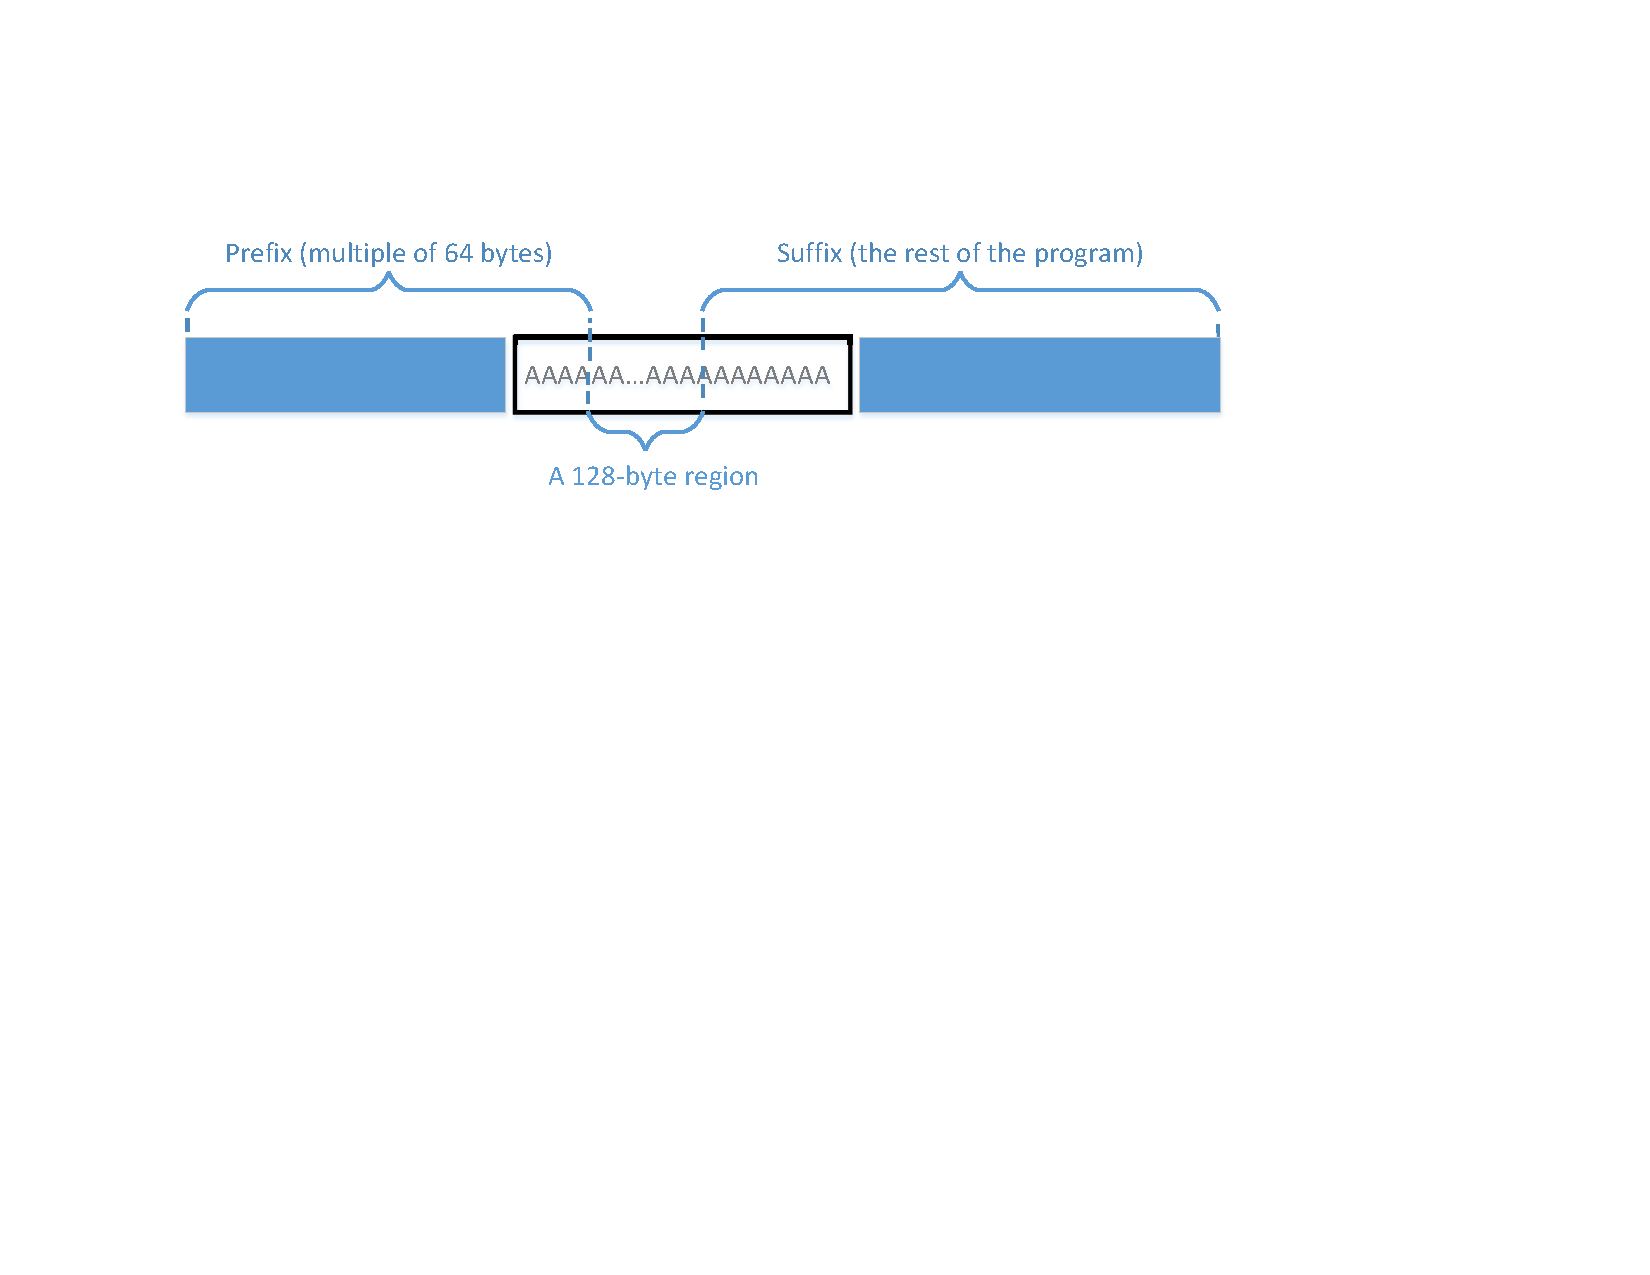
\includegraphics[width=0.9\textwidth]{\mdFigs/fill_array.pdf}
\end{center}
\caption{Break the executable file into three pieces.}
\label{md5:fig:fill_array}
\end{figure}
 
We can run \texttt{md5collgen} on the prefix to generate 
two outputs that have the same MD5 hash value.
Let us use \texttt{P} and \texttt{Q} to represent the 
second part (each having 128 bytes) of these outputs (i.e., the part after the prefix). 
Therefore, we have the following:

\begin{lstlisting}
MD5 (prefix (*@$\|$@*) P) = MD5 (prefix (*@$\|$@*) Q)
\end{lstlisting}

Based on the property of MD5, we know that if we append the same suffix to 
the above two outputs, the resultant data will also have the 
same hash value. Basically, the following is true for any suffix:

\begin{lstlisting}
MD5 (prefix (*@$\|$@*) P (*@$\|$@*) suffix) = MD5 (prefix (*@$\|$@*) Q (*@$\|$@*) suffix)
\end{lstlisting}

Therefore, we just need to use \texttt{P} and \texttt{Q} to replace 
128 bytes of the array (between the two dividing points), and we will be able to
create two binary programs that have the same hash value. 
Their outcomes are different, because they each print out their own arrays, which have
different contents. 


\paragraph{Tools.} You can use \texttt{bless}
to view the binary executable file and find the location for the 
array. For dividing a binary file, there are some 
tools that we can use to 
divide a file from a particular location. The \texttt{head} 
and \texttt{tail} commands are such useful tools. 
You can look at their manuals to
learn how to use them. We give three examples in the following:  

\begin{lstlisting}
$ head -c 3200 a.out > prefix
$ tail -c 100 a.out > suffix
$ tail -c +3300 a.out > suffix
\end{lstlisting}

The first command above saves the first \texttt{3200} bytes
of \texttt{a.out} to \texttt{prefix}. The second command 
saves the last \texttt{100} bytes of \texttt{a.out} 
to \texttt{suffix}. The third command 
saves the data from the \texttt{3300}th byte to the end of   
the file \texttt{a.out} to \texttt{suffix}.  With these two
commands, we can divide a binary file into pieces from 
any location. If we need to glue some pieces together, we can 
use the \texttt{cat} command.  


If you use \texttt{bless} to copy-and-paste a block of data from one binary file to another file, the
menu item \texttt{"Edit -> Select Range"} is quite handy, because you can select 
a block of data using a starting point and a range, instead of manually counting how 
many bytes are selected. 




% -------------------------------------------
% SUBSECTION
% ------------------------------------------- 
\subsection{Task 4: Making the Two Programs Behave Differently}

In the previous task, we have successfully created two programs
that have the same MD5 hash, but their behaviors are different. 
However, their differences are only in the data they print out; they 
still execute the same sequence of instructions.  
In this task, we would like to achieve something more significant 
and more meaningful. 


Assume that you have created a software which does good things.
You send the software to a trusted authority to get certified. The authority
conducts a comprehensive testing of your software, and concludes that
your software is indeed doing good things. The authority 
will present you with a certificate, stating that your program
is good. To prevent you from changing your program after getting the certificate, the 
MD5 hash value of your program is also included in the certificate; the certificate is 
signed by the authority, so you cannot change anything on the certificate or
your program without rendering the signature invalid. 



You would like to get your malicious software certified by the authority, but you have zero
chance to achieve that goal if you simply send your malicious software to the authority. 
However, you have noticed that the authority uses MD5 to generate the hash value. You
got an idea. You plan 
to prepare two different programs. One program will always execute benign instructions and do
good things, while the other program will execute malicious instructions and cause damages. 
You find a way to get these two programs to share the same MD5 hash value. 


You then send the benign version to the authority for certification. Since this version
does good things, it will pass the certification, and you will get a certificate
that contains the hash value of your benign program. Because your malicious program has the
same hash value, this certificate is also valid for your malicious program. Therefore, you have
successfully obtained a valid certificate for your malicious program. If other people trusted
the certificate issued by the authority, they will download your malicious program. 


\underline{The objective of this task} is to launch the attack described above. 
Namely, you need to create two programs that 
share the same MD5 hash. However, one program
will always execute benign instructions, while the other program will 
execute malicious instructions. In your work, what benign/malicious instructions are 
executed is not important; it is sufficient to demonstrate that the
instructions executed by these two programs are different. 



\paragraph{Guidelines.}
Creating two completely different programs that produce the same MD5 hash value is quite hard.
The two hash-colliding programs produced by \texttt{md5collgen} need to share the same prefix;
moreover, as we can see from the previous task, if we need to add some meaningful suffix 
to the outputs produced by \texttt{md5collgen}, the suffix added to both 
programs also needs to be the same. These are the limitations of the 
MD5 collision generation program that we use. 
Although there are other more complicated and more advanced tools that can lift some of the
limitations, such as accepting two different prefixes~\cite{stevens2007}, they demand much more 
computing power, so they are out of the scope for this lab. We need to find a way to 
generate two different programs within the limitations.


There are many ways to achieve the above goal. We provide one approach as a reference,
but students are encouraged to come up their own ideas. Instructors may consider rewarding
students for their own ideas. 
In our approach, we create two arrays \texttt{X} and \texttt{Y}. We
compare the contents of these two arrays; if they are the same, the benign code is executed;
otherwise, the malicious code is executed. See the following pseudo-code: 


\begin{lstlisting}
Array X;
Array Y;

main()
{
  if(X's contents and Y's contents are the same)
      run benign code;
  else
      run malicious code;
  return;
}
\end{lstlisting}


We can initialize the arrays \texttt{X} and \texttt{Y} with some values that can help us find
their locations in the executable binary file. Our job is to change the contents of
these two arrays, so we can generate two different versions that have the same MD5 hash. 
In one version, the contents of X and Y are the same, so the benign code is executed;
in the other version, the contents of X and Y are different, so the malicious code 
is executed. We can achieve this goal using a technique similar to the one used in Task 3. 
Figure~\ref{md5:fig:two_versions} illustrates what the two versions of the program look like. 

\begin{figure}[htb]
	\centering
	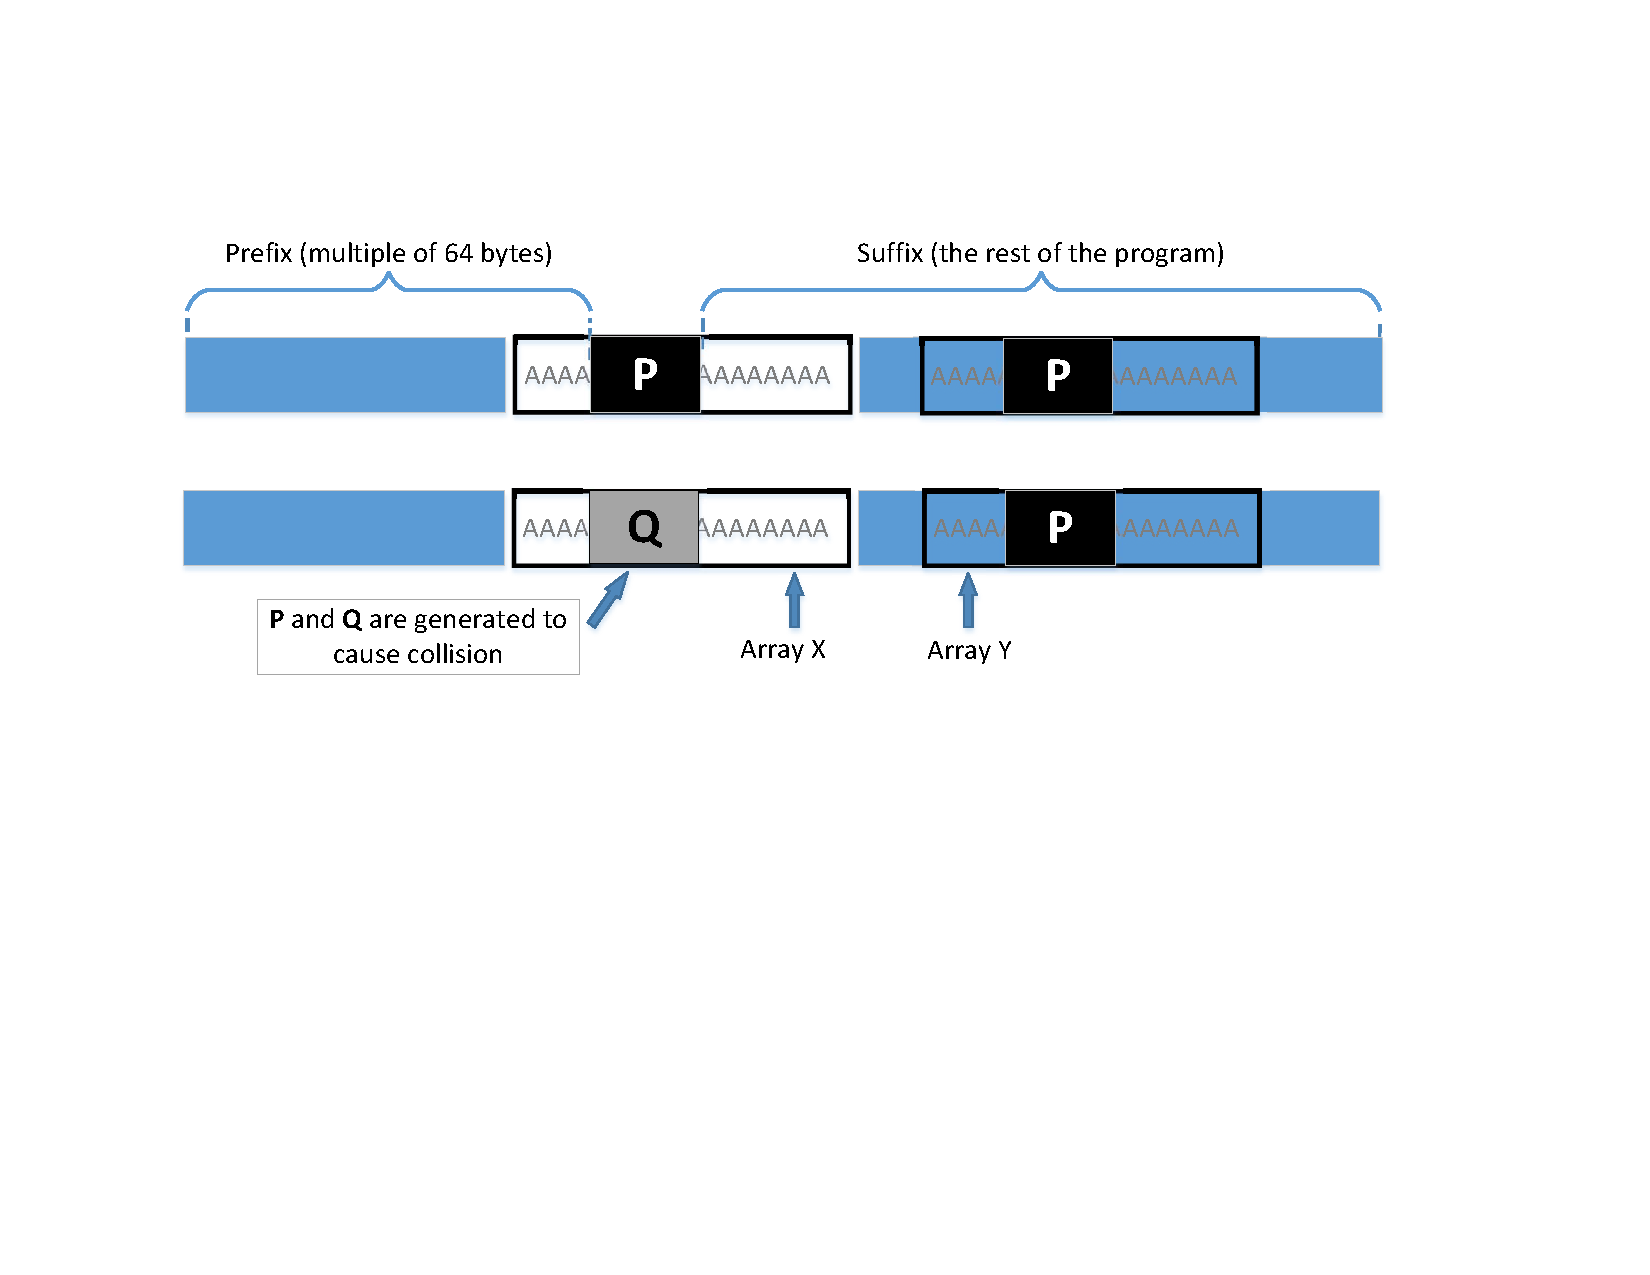
\includegraphics[width=0.9\textwidth]{\mdFigs/two_versions.pdf}
	\caption{An approach to generate two hash-colliding programs with different behaviors.}
	\label{md5:fig:two_versions}
\end{figure}

From Figure~\ref{md5:fig:two_versions}, we know that these two binary files have
the same MD5 hash value, as long as \texttt{P} and \texttt{Q} are generated accordingly. 
In the first version, we make the contents of arrays X and Y the same, while in the second
version, we make their contents different. Therefore, the only thing we need to change is the
contents of these two arrays, and there is no need to change the logic of the programs. 


%\paragraph{Questions.} After finishing this task, please answer the following questions:
%
%
%\begin{itemize}[label={--}]
%\item \textbf{Problem 5.} In Figure~\ref{md5:fig:two_versions}, can we place array \texttt{Y} in the prefix instead of
%in the suffix? Please explain. 

%\item \textbf{Problem 6.} Given an existing program made by other people, can we use the
%\texttt{md5collgen} program to create  different program that has the same value as this
%existing one?  Please explain. 
%\end{itemize}
 


% *******************************************
% SECTION
% ******************************************* 
\section{Submission}


%%%%%%%%%%%%%%%%%%%%%%%%%%%%%%%%%%%%%%%%

You need to submit a detailed lab report, with screenshots,
to describe what you have done and what you have observed.
You also need to provide explanation
to the observations that are interesting or surprising.
Please also list the important code snippets followed by
explanation. Simply attaching code without any explanation will not
receive credits.

%%%%%%%%%%%%%%%%%%%%%%%%%%%%%%%%%%%%%%%%


%%%%%%%%%%%%%%%%%%%%%%%%%%%%%%%%%%%%%%%%%%%%%%%%%%%%%%%%%%%%%%%%%%%%%%
\bibliographystyle{plain}
\def\baselinestretch{1}
\bibliography{BibMD5Lab}
%%%%%%%%%%%%%%%%%%%%%%%%%%%%%%%%%%%%%%%%%%%%%%%%%%%%%%%%%%%%%%%%%%%%%%


\end{document}
